\documentclass[1p]{elsarticle_modified}
%\bibliographystyle{elsarticle-num}

%\usepackage[colorlinks]{hyperref}
%\usepackage{abbrmath_seonhwa} %\Abb, \Ascr, \Acal ,\Abf, \Afrak
\usepackage{amsfonts}
\usepackage{amssymb}
\usepackage{amsmath}
\usepackage{amsthm}
\usepackage{scalefnt}
\usepackage{amsbsy}
\usepackage{kotex}
\usepackage{caption}
\usepackage{subfig}
\usepackage{color}
\usepackage{graphicx}
\usepackage{xcolor} %% white, black, red, green, blue, cyan, magenta, yellow
\usepackage{float}
\usepackage{setspace}
\usepackage{hyperref}

\usepackage{tikz}
\usetikzlibrary{arrows}

\usepackage{multirow}
\usepackage{array} % fixed length table
\usepackage{hhline}

%%%%%%%%%%%%%%%%%%%%%
\makeatletter
\renewcommand*\env@matrix[1][\arraystretch]{%
	\edef\arraystretch{#1}%
	\hskip -\arraycolsep
	\let\@ifnextchar\new@ifnextchar
	\array{*\c@MaxMatrixCols c}}
\makeatother %https://tex.stackexchange.com/questions/14071/how-can-i-increase-the-line-spacing-in-a-matrix
%%%%%%%%%%%%%%%

\usepackage[normalem]{ulem}

\newcommand{\msout}[1]{\ifmmode\text{\sout{\ensuremath{#1}}}\else\sout{#1}\fi}
%SOURCE: \msout is \stkout macro in https://tex.stackexchange.com/questions/20609/strikeout-in-math-mode

\newcommand{\cancel}[1]{
	\ifmmode
	{\color{red}\msout{#1}}
	\else
	{\color{red}\sout{#1}}
	\fi
}

\newcommand{\add}[1]{
	{\color{blue}\uwave{#1}}
}

\newcommand{\replace}[2]{
	\ifmmode
	{\color{red}\msout{#1}}{\color{blue}\uwave{#2}}
	\else
	{\color{red}\sout{#1}}{\color{blue}\uwave{#2}}
	\fi
}

\newcommand{\Sol}{\mathcal{S}} %segment
\newcommand{\D}{D} %diagram
\newcommand{\A}{\mathcal{A}} %arc


%%%%%%%%%%%%%%%%%%%%%%%%%%%%%5 test

\def\sl{\operatorname{\textup{SL}}(2,\Cbb)}
\def\psl{\operatorname{\textup{PSL}}(2,\Cbb)}
\def\quan{\mkern 1mu \triangleright \mkern 1mu}

\theoremstyle{definition}
\newtheorem{thm}{Theorem}[section]
\newtheorem{prop}[thm]{Proposition}
\newtheorem{lem}[thm]{Lemma}
\newtheorem{ques}[thm]{Question}
\newtheorem{cor}[thm]{Corollary}
\newtheorem{defn}[thm]{Definition}
\newtheorem{exam}[thm]{Example}
\newtheorem{rmk}[thm]{Remark}
\newtheorem{alg}[thm]{Algorithm}

\newcommand{\I}{\sqrt{-1}}
\begin{document}

%\begin{frontmatter}
%
%\title{Boundary parabolic representations of knots up to 8 crossings}
%
%%% Group authors per affiliation:
%\author{Yunhi Cho} 
%\address{Department of Mathematics, University of Seoul, Seoul, Korea}
%\ead{yhcho@uos.ac.kr}
%
%
%\author{Seonhwa Kim} %\fnref{s_kim}}
%\address{Center for Geometry and Physics, Institute for Basic Science, Pohang, 37673, Korea}
%\ead{ryeona17@ibs.re.kr}
%
%\author{Hyuk Kim}
%\address{Department of Mathematical Sciences, Seoul National University, Seoul 08826, Korea}
%\ead{hyukkim@snu.ac.kr}
%
%\author{Seokbeom Yoon}
%\address{Department of Mathematical Sciences, Seoul National University, Seoul, 08826,  Korea}
%\ead{sbyoon15@snu.ac.kr}
%
%\begin{abstract}
%We find all boundary parabolic representation of knots up to 8 crossings.
%
%\end{abstract}
%\begin{keyword}
%    \MSC[2010] 57M25 
%\end{keyword}
%
%\end{frontmatter}

%\linenumbers
%\tableofcontents
%
\newcommand\colored[1]{\textcolor{white}{\rule[-0.35ex]{0.8em}{1.4ex}}\kern-0.8em\color{red} #1}%
%\newcommand\colored[1]{\textcolor{white}{ #1}\kern-2.17ex	\textcolor{white}{ #1}\kern-1.81ex	\textcolor{white}{ #1}\kern-2.15ex\color{red}#1	}

{\Large $\underline{12a_{0952}~(K12a_{0952})}$}

\setlength{\tabcolsep}{10pt}
\renewcommand{\arraystretch}{1.6}
\vspace{1cm}\begin{tabular}{m{100pt}>{\centering\arraybackslash}m{274pt}}
\multirow{5}{120pt}{
	\centering
	\includegraphics[width=112pt]{../../../GIT/diagram.site/Diagrams/png/1753_12a_0952.png}\\
\ \ \ A knot diagram\footnotemark}&
\allowdisplaybreaks
\textbf{Linearized knot diagam} \\
\cline{2-2}
 &
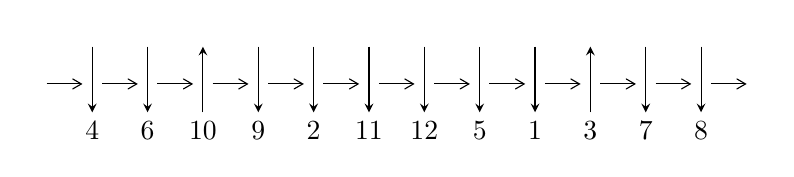
\begin{tikzpicture}[x=20pt, y=17pt]
	% nodes
	\node (C0) at (0, 0) {};
	\node (C1) at (1, 0) {};
	\node (C1U) at (1, +1) {};
	\node (C1D) at (1, -1) {4};

	\node (C2) at (2, 0) {};
	\node (C2U) at (2, +1) {};
	\node (C2D) at (2, -1) {6};

	\node (C3) at (3, 0) {};
	\node (C3U) at (3, +1) {};
	\node (C3D) at (3, -1) {10};

	\node (C4) at (4, 0) {};
	\node (C4U) at (4, +1) {};
	\node (C4D) at (4, -1) {9};

	\node (C5) at (5, 0) {};
	\node (C5U) at (5, +1) {};
	\node (C5D) at (5, -1) {2};

	\node (C6) at (6, 0) {};
	\node (C6U) at (6, +1) {};
	\node (C6D) at (6, -1) {11};

	\node (C7) at (7, 0) {};
	\node (C7U) at (7, +1) {};
	\node (C7D) at (7, -1) {12};

	\node (C8) at (8, 0) {};
	\node (C8U) at (8, +1) {};
	\node (C8D) at (8, -1) {5};

	\node (C9) at (9, 0) {};
	\node (C9U) at (9, +1) {};
	\node (C9D) at (9, -1) {1};

	\node (C10) at (10, 0) {};
	\node (C10U) at (10, +1) {};
	\node (C10D) at (10, -1) {3};

	\node (C11) at (11, 0) {};
	\node (C11U) at (11, +1) {};
	\node (C11D) at (11, -1) {7};

	\node (C12) at (12, 0) {};
	\node (C12U) at (12, +1) {};
	\node (C12D) at (12, -1) {8};
	\node (C13) at (13, 0) {};

	% arrows
	\draw[->,>={angle 60}]
	(C0) edge (C1) (C1) edge (C2) (C2) edge (C3) (C3) edge (C4) (C4) edge (C5) (C5) edge (C6) (C6) edge (C7) (C7) edge (C8) (C8) edge (C9) (C9) edge (C10) (C10) edge (C11) (C11) edge (C12) (C12) edge (C13) ;	\draw[->,>=stealth]
	(C1U) edge (C1D) (C2U) edge (C2D) (C3D) edge (C3U) (C4U) edge (C4D) (C5U) edge (C5D) (C6U) edge (C6D) (C7U) edge (C7D) (C8U) edge (C8D) (C9U) edge (C9D) (C10D) edge (C10U) (C11U) edge (C11D) (C12U) edge (C12D) ;
	\end{tikzpicture} \\
\hhline{~~} \\& 
\textbf{Solving Sequence} \\ \cline{2-2} 
 &
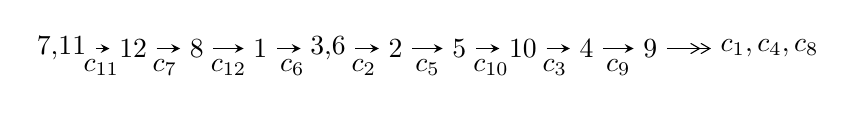
\begin{tikzpicture}[x=23pt, y=7pt]
	% node
	\node (A0) at (-1/8, 0) {7,11};
	\node (A1) at (1, 0) {12};
	\node (A2) at (2, 0) {8};
	\node (A3) at (3, 0) {1};
	\node (A4) at (65/16, 0) {3,6};
	\node (A5) at (41/8, 0) {2};
	\node (A6) at (49/8, 0) {5};
	\node (A7) at (57/8, 0) {10};
	\node (A8) at (65/8, 0) {4};
	\node (A9) at (73/8, 0) {9};
	\node (C1) at (1/2, -1) {$c_{11}$};
	\node (C2) at (3/2, -1) {$c_{7}$};
	\node (C3) at (5/2, -1) {$c_{12}$};
	\node (C4) at (7/2, -1) {$c_{6}$};
	\node (C5) at (37/8, -1) {$c_{2}$};
	\node (C6) at (45/8, -1) {$c_{5}$};
	\node (C7) at (53/8, -1) {$c_{10}$};
	\node (C8) at (61/8, -1) {$c_{3}$};
	\node (C9) at (69/8, -1) {$c_{9}$};
	\node (A10) at (11, 0) {$c_{1},c_{4},c_{8}$};

	% edge
	\draw[->,>=stealth]	
	(A0) edge (A1) (A1) edge (A2) (A2) edge (A3) (A3) edge (A4) (A4) edge (A5) (A5) edge (A6) (A6) edge (A7) (A7) edge (A8) (A8) edge (A9) ;
	\draw[->>,>={angle 60}]	
	(A9) edge (A10);
\end{tikzpicture} \\ 

\end{tabular} \\

\footnotetext{
The image of knot diagram is generated by the software ``\textbf{Draw programme}" developed by Andrew Bartholomew(\url{http://www.layer8.co.uk/maths/draw/index.htm\#Running-draw}), where we modified some parts for our purpose(\url{https://github.com/CATsTAILs/LinksPainter}).
}\phantom \\ \newline 
\centering \textbf{Ideals for irreducible components\footnotemark of $X_{\text{par}}$} 
 
\begin{align*}
I^u_{1}&=\langle 
-4.06116\times10^{117} u^{76}+8.53092\times10^{117} u^{75}+\cdots+9.26283\times10^{117} b+6.65560\times10^{118},\\
\phantom{I^u_{1}}&\phantom{= \langle  }-1.56367\times10^{119} u^{76}+2.54497\times10^{120} u^{75}+\cdots+1.20232\times10^{121} a-2.34026\times10^{122},\\
\phantom{I^u_{1}}&\phantom{= \langle  }u^{77}- u^{76}+\cdots-267 u-11\rangle \\
I^u_{2}&=\langle 
u^7-5 u^5+u^4+7 u^3-3 u^2+b-2 u+1,\;u^7-5 u^5+u^4+7 u^3-4 u^2+a-2 u+3,\\
\phantom{I^u_{2}}&\phantom{= \langle  }u^{14}-10 u^{12}+2 u^{11}+39 u^{10}-16 u^9-73 u^8+46 u^7+63 u^6-56 u^5-17 u^4+25 u^3-2 u^2-2 u+1\rangle \\
I^u_{3}&=\langle 
b- a-1,\;a^2+a+1,\;u+1\rangle \\
\\
\end{align*}
\raggedright * 3 irreducible components of $\dim_{\mathbb{C}}=0$, with total 93 representations.\\
\footnotetext{All coefficients of polynomials are rational numbers. But the coefficients are sometimes approximated in decimal forms when there is not enough margin.}
\newpage
\renewcommand{\arraystretch}{1}
\centering \section*{I. $I^u_{1}= \langle -4.06\times10^{117} u^{76}+8.53\times10^{117} u^{75}+\cdots+9.26\times10^{117} b+6.66\times10^{118},\;-1.56\times10^{119} u^{76}+2.54\times10^{120} u^{75}+\cdots+1.20\times10^{121} a-2.34\times10^{122},\;u^{77}- u^{76}+\cdots-267 u-11 \rangle$}
\flushleft \textbf{(i) Arc colorings}\\
\begin{tabular}{m{7pt} m{180pt} m{7pt} m{180pt} }
\flushright $a_{7}=$&$\begin{pmatrix}0\\u\end{pmatrix}$ \\
\flushright $a_{11}=$&$\begin{pmatrix}1\\0\end{pmatrix}$ \\
\flushright $a_{12}=$&$\begin{pmatrix}1\\u^2\end{pmatrix}$ \\
\flushright $a_{8}=$&$\begin{pmatrix}- u\\- u^3+u\end{pmatrix}$ \\
\flushright $a_{1}=$&$\begin{pmatrix}- u^2+1\\- u^4+2 u^2\end{pmatrix}$ \\
\flushright $a_{3}=$&$\begin{pmatrix}0.0130055 u^{76}-0.211672 u^{75}+\cdots+76.4038 u+19.4646\\0.438436 u^{76}-0.920984 u^{75}+\cdots-179.356 u-7.18528\end{pmatrix}$ \\
\flushright $a_{6}=$&$\begin{pmatrix}u\\u\end{pmatrix}$ \\
\flushright $a_{2}=$&$\begin{pmatrix}0.167907 u^{76}-0.560036 u^{75}+\cdots+5.28710 u+16.3419\\0.593337 u^{76}-1.26935 u^{75}+\cdots-250.473 u-10.3080\end{pmatrix}$ \\
\flushright $a_{5}=$&$\begin{pmatrix}-0.411584 u^{76}+0.826205 u^{75}+\cdots+35.9924 u-12.3201\\-0.626576 u^{76}+1.06289 u^{75}+\cdots+236.498 u+9.82640\end{pmatrix}$ \\
\flushright $a_{10}=$&$\begin{pmatrix}-0.367850 u^{76}+0.345807 u^{75}+\cdots+92.0501 u+14.7008\\-1.23947 u^{76}+1.85355 u^{75}+\cdots+320.091 u+14.3520\end{pmatrix}$ \\
\flushright $a_{4}=$&$\begin{pmatrix}0.210003 u^{76}-1.23021 u^{75}+\cdots-8.76425 u+22.4581\\1.40382 u^{76}-3.36880 u^{75}+\cdots-583.635 u-24.2823\end{pmatrix}$ \\
\flushright $a_{9}=$&$\begin{pmatrix}-0.449798 u^{76}+0.574876 u^{75}+\cdots+146.822 u+17.4073\\-1.28744 u^{76}+2.03905 u^{75}+\cdots+374.165 u+16.7057\end{pmatrix}$\\&\end{tabular}
\flushleft \textbf{(ii) Obstruction class $= -1$}\\~\\
\flushleft \textbf{(iii) Cusp Shapes $= -10.0222 u^{76}+16.2318 u^{75}+\cdots+3664.59 u+156.514$}\\~\\
\newpage\renewcommand{\arraystretch}{1}
\flushleft \textbf{(iv) u-Polynomials at the component}\newline \\
\begin{tabular}{m{50pt}|m{274pt}}
Crossings & \hspace{64pt}u-Polynomials at each crossing \\
\hline $$\begin{aligned}c_{1}\end{aligned}$$&$\begin{aligned}
&u^{77}-9 u^{76}+\cdots-22 u+1
\end{aligned}$\\
\hline $$\begin{aligned}c_{2},c_{5}\end{aligned}$$&$\begin{aligned}
&u^{77}+u^{76}+\cdots+6201 u+108
\end{aligned}$\\
\hline $$\begin{aligned}c_{3},c_{10}\end{aligned}$$&$\begin{aligned}
&u^{77}+33 u^{75}+\cdots-4491 u-361
\end{aligned}$\\
\hline $$\begin{aligned}c_{4},c_{8}\end{aligned}$$&$\begin{aligned}
&u^{77}+3 u^{76}+\cdots-368 u-79
\end{aligned}$\\
\hline $$\begin{aligned}c_{6},c_{7},c_{11}\\c_{12}\end{aligned}$$&$\begin{aligned}
&u^{77}- u^{76}+\cdots-267 u-11
\end{aligned}$\\
\hline $$\begin{aligned}c_{9}\end{aligned}$$&$\begin{aligned}
&u^{77}+6 u^{76}+\cdots+12 u+8
\end{aligned}$\\
\hline
\end{tabular}\\~\\
\newpage\renewcommand{\arraystretch}{1}
\flushleft \textbf{(v) Riley Polynomials at the component}\newline \\
\begin{tabular}{m{50pt}|m{274pt}}
Crossings & \hspace{64pt}Riley Polynomials at each crossing \\
\hline $$\begin{aligned}c_{1}\end{aligned}$$&$\begin{aligned}
&y^{77}-5 y^{76}+\cdots+70 y-1
\end{aligned}$\\
\hline $$\begin{aligned}c_{2},c_{5}\end{aligned}$$&$\begin{aligned}
&y^{77}-73 y^{76}+\cdots+14541849 y-11664
\end{aligned}$\\
\hline $$\begin{aligned}c_{3},c_{10}\end{aligned}$$&$\begin{aligned}
&y^{77}+66 y^{76}+\cdots+8226479 y-130321
\end{aligned}$\\
\hline $$\begin{aligned}c_{4},c_{8}\end{aligned}$$&$\begin{aligned}
&y^{77}+35 y^{76}+\cdots-116112 y-6241
\end{aligned}$\\
\hline $$\begin{aligned}c_{6},c_{7},c_{11}\\c_{12}\end{aligned}$$&$\begin{aligned}
&y^{77}-99 y^{76}+\cdots+37057 y-121
\end{aligned}$\\
\hline $$\begin{aligned}c_{9}\end{aligned}$$&$\begin{aligned}
&y^{77}-12 y^{76}+\cdots+2032 y-64
\end{aligned}$\\
\hline
\end{tabular}\\~\\
\newpage\flushleft \textbf{(vi) Complex Volumes and Cusp Shapes}
$$\begin{array}{c|c|c}  
\text{Solutions to }I^u_{1}& \I (\text{vol} + \sqrt{-1}CS) & \text{Cusp shape}\\
 \hline 
\begin{aligned}
u &= \phantom{-}0.038185 + 0.977495 I \\
a &= -0.0887050 - 0.0211649 I \\
b &= \phantom{-}0.180623 - 1.401330 I\end{aligned}
 & -3.38576 - 7.06554 I & \phantom{-0.000000 } 0 \\ \hline\begin{aligned}
u &= \phantom{-}0.038185 - 0.977495 I \\
a &= -0.0887050 + 0.0211649 I \\
b &= \phantom{-}0.180623 + 1.401330 I\end{aligned}
 & -3.38576 + 7.06554 I & \phantom{-0.000000 } 0 \\ \hline\begin{aligned}
u &= \phantom{-}0.959703 + 0.096825 I \\
a &= -0.20377 - 1.90119 I \\
b &= \phantom{-}0.228834 - 1.133660 I\end{aligned}
 & -4.11267 - 2.60144 I & \phantom{-0.000000 } 0 \\ \hline\begin{aligned}
u &= \phantom{-}0.959703 - 0.096825 I \\
a &= -0.20377 + 1.90119 I \\
b &= \phantom{-}0.228834 + 1.133660 I\end{aligned}
 & -4.11267 + 2.60144 I & \phantom{-0.000000 } 0 \\ \hline\begin{aligned}
u &= \phantom{-}1.005850 + 0.248662 I \\
a &= -1.40505 - 1.62886 I \\
b &= \phantom{-}0.109475 - 1.292590 I\end{aligned}
 & -6.11081 - 3.61083 I & \phantom{-0.000000 } 0 \\ \hline\begin{aligned}
u &= \phantom{-}1.005850 - 0.248662 I \\
a &= -1.40505 + 1.62886 I \\
b &= \phantom{-}0.109475 + 1.292590 I\end{aligned}
 & -6.11081 + 3.61083 I & \phantom{-0.000000 } 0 \\ \hline\begin{aligned}
u &= -1.051160 + 0.193722 I \\
a &= -0.588531 - 0.688350 I \\
b &= \phantom{-}0.226875 - 0.069667 I\end{aligned}
 & -1.83333 - 1.94928 I & \phantom{-0.000000 } 0 \\ \hline\begin{aligned}
u &= -1.051160 - 0.193722 I \\
a &= -0.588531 + 0.688350 I \\
b &= \phantom{-}0.226875 + 0.069667 I\end{aligned}
 & -1.83333 + 1.94928 I & \phantom{-0.000000 } 0 \\ \hline\begin{aligned}
u &= \phantom{-}0.982142 + 0.468578 I \\
a &= \phantom{-}0.91609 + 1.21859 I \\
b &= -0.39039 + 1.53681 I\end{aligned}
 & -9.70005 - 6.50940 I & \phantom{-0.000000 } 0 \\ \hline\begin{aligned}
u &= \phantom{-}0.982142 - 0.468578 I \\
a &= \phantom{-}0.91609 - 1.21859 I \\
b &= -0.39039 - 1.53681 I\end{aligned}
 & -9.70005 + 6.50940 I & \phantom{-0.000000 } 0\\
 \hline 
 \end{array}$$\newpage$$\begin{array}{c|c|c}  
\text{Solutions to }I^u_{1}& \I (\text{vol} + \sqrt{-1}CS) & \text{Cusp shape}\\
 \hline 
\begin{aligned}
u &= -0.766904 + 0.773981 I \\
a &= -0.921347 + 0.489206 I \\
b &= \phantom{-}0.091213 + 1.388450 I\end{aligned}
 & -7.58242 + 2.37767 I & \phantom{-0.000000 } 0 \\ \hline\begin{aligned}
u &= -0.766904 - 0.773981 I \\
a &= -0.921347 - 0.489206 I \\
b &= \phantom{-}0.091213 - 1.388450 I\end{aligned}
 & -7.58242 - 2.37767 I & \phantom{-0.000000 } 0 \\ \hline\begin{aligned}
u &= \phantom{-}0.830594 + 0.329150 I \\
a &= \phantom{-}0.253500 + 0.255718 I \\
b &= -1.058950 + 0.357207 I\end{aligned}
 & -0.60061 - 7.40607 I & \phantom{-0.000000 } 0 \\ \hline\begin{aligned}
u &= \phantom{-}0.830594 - 0.329150 I \\
a &= \phantom{-}0.253500 - 0.255718 I \\
b &= -1.058950 - 0.357207 I\end{aligned}
 & -0.60061 + 7.40607 I & \phantom{-0.000000 } 0 \\ \hline\begin{aligned}
u &= -0.821582 + 0.262973 I \\
a &= -0.40258 + 2.54715 I \\
b &= \phantom{-}0.246547 + 1.190120 I\end{aligned}
 & -1.06852 + 6.57872 I & \phantom{-0.000000 } 0 \\ \hline\begin{aligned}
u &= -0.821582 - 0.262973 I \\
a &= -0.40258 - 2.54715 I \\
b &= \phantom{-}0.246547 - 1.190120 I\end{aligned}
 & -1.06852 - 6.57872 I & \phantom{-0.000000 } 0 \\ \hline\begin{aligned}
u &= -1.002280 + 0.636861 I \\
a &= \phantom{-}0.88637 - 1.12933 I \\
b &= -0.36459 - 1.49562 I\end{aligned}
 & -6.57021 + 12.38620 I & \phantom{-0.000000 } 0 \\ \hline\begin{aligned}
u &= -1.002280 - 0.636861 I \\
a &= \phantom{-}0.88637 + 1.12933 I \\
b &= -0.36459 + 1.49562 I\end{aligned}
 & -6.57021 - 12.38620 I & \phantom{-0.000000 } 0 \\ \hline\begin{aligned}
u &= -1.241390 + 0.072237 I \\
a &= -0.175685 + 0.764416 I \\
b &= \phantom{-}0.482561 + 0.410258 I\end{aligned}
 & -1.57748 + 1.98475 I & \phantom{-0.000000 } 0 \\ \hline\begin{aligned}
u &= -1.241390 - 0.072237 I \\
a &= -0.175685 - 0.764416 I \\
b &= \phantom{-}0.482561 - 0.410258 I\end{aligned}
 & -1.57748 - 1.98475 I & \phantom{-0.000000 } 0\\
 \hline 
 \end{array}$$\newpage$$\begin{array}{c|c|c}  
\text{Solutions to }I^u_{1}& \I (\text{vol} + \sqrt{-1}CS) & \text{Cusp shape}\\
 \hline 
\begin{aligned}
u &= -0.177425 + 0.729527 I \\
a &= -0.364310 - 0.428903 I \\
b &= \phantom{-}0.162031 + 1.383920 I\end{aligned}
 & -6.18457 + 2.49771 I & -14.4448 + 0. I\phantom{ +0.000000I} \\ \hline\begin{aligned}
u &= -0.177425 - 0.729527 I \\
a &= -0.364310 + 0.428903 I \\
b &= \phantom{-}0.162031 - 1.383920 I\end{aligned}
 & -6.18457 - 2.49771 I & -14.4448 + 0. I\phantom{ +0.000000I} \\ \hline\begin{aligned}
u &= \phantom{-}0.582280 + 0.471981 I \\
a &= \phantom{-}0.168635 - 0.799555 I \\
b &= \phantom{-}0.574579 + 0.079542 I\end{aligned}
 & \phantom{-}2.28027 - 3.59748 I & -8.00000 + 4.60742 I \\ \hline\begin{aligned}
u &= \phantom{-}0.582280 - 0.471981 I \\
a &= \phantom{-}0.168635 + 0.799555 I \\
b &= \phantom{-}0.574579 - 0.079542 I\end{aligned}
 & \phantom{-}2.28027 + 3.59748 I & -8.00000 - 4.60742 I \\ \hline\begin{aligned}
u &= \phantom{-}0.693292 + 0.271817 I \\
a &= -1.153550 + 0.702978 I \\
b &= \phantom{-}0.344954 - 0.059152 I\end{aligned}
 & -2.76074 - 0.90392 I & -8.00000 + 8.29169 I \\ \hline\begin{aligned}
u &= \phantom{-}0.693292 - 0.271817 I \\
a &= -1.153550 - 0.702978 I \\
b &= \phantom{-}0.344954 + 0.059152 I\end{aligned}
 & -2.76074 + 0.90392 I & -8.00000 - 8.29169 I \\ \hline\begin{aligned}
u &= -0.733460 + 0.065281 I \\
a &= -0.382545 - 1.223710 I \\
b &= -1.83460 - 1.32389 I\end{aligned}
 & -2.96946 + 0.15069 I & \phantom{-}50.9420 - 6.6243 I \\ \hline\begin{aligned}
u &= -0.733460 - 0.065281 I \\
a &= -0.382545 + 1.223710 I \\
b &= -1.83460 + 1.32389 I\end{aligned}
 & -2.96946 - 0.15069 I & \phantom{-}50.9420 + 6.6243 I \\ \hline\begin{aligned}
u &= -0.698952 + 0.210701 I \\
a &= -2.35802 + 0.99441 I \\
b &= \phantom{-}0.121661 + 1.318110 I\end{aligned}
 & -6.82768 + 0.82988 I & -17.2416 + 2.2447 I \\ \hline\begin{aligned}
u &= -0.698952 - 0.210701 I \\
a &= -2.35802 - 0.99441 I \\
b &= \phantom{-}0.121661 - 1.318110 I\end{aligned}
 & -6.82768 - 0.82988 I & -17.2416 - 2.2447 I\\
 \hline 
 \end{array}$$\newpage$$\begin{array}{c|c|c}  
\text{Solutions to }I^u_{1}& \I (\text{vol} + \sqrt{-1}CS) & \text{Cusp shape}\\
 \hline 
\begin{aligned}
u &= \phantom{-}1.255700 + 0.237415 I \\
a &= \phantom{-}0.056230 + 1.165950 I \\
b &= \phantom{-}0.446841 + 1.052400 I\end{aligned}
 & -3.35743 + 1.81897 I & \phantom{-0.000000 } 0 \\ \hline\begin{aligned}
u &= \phantom{-}1.255700 - 0.237415 I \\
a &= \phantom{-}0.056230 - 1.165950 I \\
b &= \phantom{-}0.446841 - 1.052400 I\end{aligned}
 & -3.35743 - 1.81897 I & \phantom{-0.000000 } 0 \\ \hline\begin{aligned}
u &= \phantom{-}1.073990 + 0.741345 I \\
a &= -0.808228 - 0.841791 I \\
b &= \phantom{-}0.033391 - 1.383920 I\end{aligned}
 & -6.40287 + 1.28578 I & \phantom{-0.000000 } 0 \\ \hline\begin{aligned}
u &= \phantom{-}1.073990 - 0.741345 I \\
a &= -0.808228 + 0.841791 I \\
b &= \phantom{-}0.033391 + 1.383920 I\end{aligned}
 & -6.40287 - 1.28578 I & \phantom{-0.000000 } 0 \\ \hline\begin{aligned}
u &= -0.629004 + 0.287209 I \\
a &= \phantom{-}0.96669 - 1.28469 I \\
b &= \phantom{-}0.289074 - 1.108480 I\end{aligned}
 & -1.49663 + 0.99559 I & -12.39912 - 2.84502 I \\ \hline\begin{aligned}
u &= -0.629004 - 0.287209 I \\
a &= \phantom{-}0.96669 + 1.28469 I \\
b &= \phantom{-}0.289074 + 1.108480 I\end{aligned}
 & -1.49663 - 0.99559 I & -12.39912 + 2.84502 I \\ \hline\begin{aligned}
u &= \phantom{-}0.282100 + 0.527030 I \\
a &= \phantom{-}0.630239 + 0.170161 I \\
b &= -0.633562 + 0.251400 I\end{aligned}
 & \phantom{-}3.14780 + 0.17045 I & -2.65284 + 2.77130 I \\ \hline\begin{aligned}
u &= \phantom{-}0.282100 - 0.527030 I \\
a &= \phantom{-}0.630239 - 0.170161 I \\
b &= -0.633562 - 0.251400 I\end{aligned}
 & \phantom{-}3.14780 - 0.17045 I & -2.65284 - 2.77130 I \\ \hline\begin{aligned}
u &= -0.560530\phantom{ +0.000000I} \\
a &= \phantom{-}0.504531\phantom{ +0.000000I} \\
b &= \phantom{-}0.446354\phantom{ +0.000000I}\end{aligned}
 & -0.920531\phantom{ +0.000000I} & -10.2400\phantom{ +0.000000I} \\ \hline\begin{aligned}
u &= \phantom{-}0.077893 + 0.515289 I \\
a &= -0.22039 - 1.76338 I \\
b &= \phantom{-}0.537309 + 0.147685 I\end{aligned}
 & \phantom{-}1.69633 + 4.51493 I & -4.07565 - 3.55592 I\\
 \hline 
 \end{array}$$\newpage$$\begin{array}{c|c|c}  
\text{Solutions to }I^u_{1}& \I (\text{vol} + \sqrt{-1}CS) & \text{Cusp shape}\\
 \hline 
\begin{aligned}
u &= \phantom{-}0.077893 - 0.515289 I \\
a &= -0.22039 + 1.76338 I \\
b &= \phantom{-}0.537309 - 0.147685 I\end{aligned}
 & \phantom{-}1.69633 - 4.51493 I & -4.07565 + 3.55592 I \\ \hline\begin{aligned}
u &= -0.253806 + 0.423399 I \\
a &= \phantom{-}1.79739 + 0.32795 I \\
b &= \phantom{-}0.17927 - 1.41337 I\end{aligned}
 & -2.23223 + 1.30516 I & -8.70846 + 0.00114 I \\ \hline\begin{aligned}
u &= -0.253806 - 0.423399 I \\
a &= \phantom{-}1.79739 - 0.32795 I \\
b &= \phantom{-}0.17927 + 1.41337 I\end{aligned}
 & -2.23223 - 1.30516 I & -8.70846 - 0.00114 I \\ \hline\begin{aligned}
u &= -0.148906 + 0.435693 I \\
a &= \phantom{-}0.851093 + 0.698214 I \\
b &= -0.453634 + 1.011480 I\end{aligned}
 & \phantom{-}1.00193 - 4.19580 I & -5.61939 + 0.53554 I \\ \hline\begin{aligned}
u &= -0.148906 - 0.435693 I \\
a &= \phantom{-}0.851093 - 0.698214 I \\
b &= -0.453634 - 1.011480 I\end{aligned}
 & \phantom{-}1.00193 + 4.19580 I & -5.61939 - 0.53554 I \\ \hline\begin{aligned}
u &= -1.54899 + 0.13119 I \\
a &= -0.458921 - 0.532312 I \\
b &= -0.453875 - 0.087559 I\end{aligned}
 & -4.84668 + 5.75436 I & \phantom{-0.000000 } 0 \\ \hline\begin{aligned}
u &= -1.54899 - 0.13119 I \\
a &= -0.458921 + 0.532312 I \\
b &= -0.453875 + 0.087559 I\end{aligned}
 & -4.84668 - 5.75436 I & \phantom{-0.000000 } 0 \\ \hline\begin{aligned}
u &= \phantom{-}1.56208\phantom{ +0.000000I} \\
a &= -0.744675\phantom{ +0.000000I} \\
b &= -0.707392\phantom{ +0.000000I}\end{aligned}
 & -8.21010\phantom{ +0.000000I} & \phantom{-0.000000 } 0 \\ \hline\begin{aligned}
u &= -0.194765 + 0.328946 I \\
a &= \phantom{-}0.927094 - 0.543449 I \\
b &= -0.274652 - 0.797432 I\end{aligned}
 & -0.550057 + 1.180680 I & -6.71434 - 6.33000 I \\ \hline\begin{aligned}
u &= -0.194765 - 0.328946 I \\
a &= \phantom{-}0.927094 + 0.543449 I \\
b &= -0.274652 + 0.797432 I\end{aligned}
 & -0.550057 - 1.180680 I & -6.71434 + 6.33000 I\\
 \hline 
 \end{array}$$\newpage$$\begin{array}{c|c|c}  
\text{Solutions to }I^u_{1}& \I (\text{vol} + \sqrt{-1}CS) & \text{Cusp shape}\\
 \hline 
\begin{aligned}
u &= \phantom{-}1.63594 + 0.07265 I \\
a &= -0.49221 - 2.03787 I \\
b &= -0.21035 - 1.56875 I\end{aligned}
 & -9.51163 - 2.28865 I & \phantom{-0.000000 } 0 \\ \hline\begin{aligned}
u &= \phantom{-}1.63594 - 0.07265 I \\
a &= -0.49221 + 2.03787 I \\
b &= -0.21035 + 1.56875 I\end{aligned}
 & -9.51163 + 2.28865 I & \phantom{-0.000000 } 0 \\ \hline\begin{aligned}
u &= \phantom{-}1.65591 + 0.01982 I \\
a &= \phantom{-}1.12708 - 1.41391 I \\
b &= \phantom{-}1.88510 - 1.34051 I\end{aligned}
 & -11.46620 - 0.48828 I & \phantom{-0.000000 } 0 \\ \hline\begin{aligned}
u &= \phantom{-}1.65591 - 0.01982 I \\
a &= \phantom{-}1.12708 + 1.41391 I \\
b &= \phantom{-}1.88510 + 1.34051 I\end{aligned}
 & -11.46620 + 0.48828 I & \phantom{-0.000000 } 0 \\ \hline\begin{aligned}
u &= -1.65428 + 0.07783 I \\
a &= \phantom{-}0.140794 + 0.057576 I \\
b &= -0.803163 - 0.072746 I\end{aligned}
 & -11.09700 + 2.25616 I & \phantom{-0.000000 } 0 \\ \hline\begin{aligned}
u &= -1.65428 - 0.07783 I \\
a &= \phantom{-}0.140794 - 0.057576 I \\
b &= -0.803163 + 0.072746 I\end{aligned}
 & -11.09700 - 2.25616 I & \phantom{-0.000000 } 0 \\ \hline\begin{aligned}
u &= \phantom{-}1.65550 + 0.05326 I \\
a &= \phantom{-}0.86314 + 1.70541 I \\
b &= -0.324921 + 1.348630 I\end{aligned}
 & -15.2209 - 1.8009 I & \phantom{-0.000000 } 0 \\ \hline\begin{aligned}
u &= \phantom{-}1.65550 - 0.05326 I \\
a &= \phantom{-}0.86314 - 1.70541 I \\
b &= -0.324921 - 1.348630 I\end{aligned}
 & -15.2209 + 1.8009 I & \phantom{-0.000000 } 0 \\ \hline\begin{aligned}
u &= -1.67130 + 0.08386 I \\
a &= \phantom{-}0.571962 + 0.560598 I \\
b &= \phantom{-}1.40627 + 0.45907 I\end{aligned}
 & -9.37948 + 8.96392 I & \phantom{-0.000000 } 0 \\ \hline\begin{aligned}
u &= -1.67130 - 0.08386 I \\
a &= \phantom{-}0.571962 - 0.560598 I \\
b &= \phantom{-}1.40627 - 0.45907 I\end{aligned}
 & -9.37948 - 8.96392 I & \phantom{-0.000000 } 0\\
 \hline 
 \end{array}$$\newpage$$\begin{array}{c|c|c}  
\text{Solutions to }I^u_{1}& \I (\text{vol} + \sqrt{-1}CS) & \text{Cusp shape}\\
 \hline 
\begin{aligned}
u &= \phantom{-}1.67370 + 0.06775 I \\
a &= \phantom{-}0.03577 + 2.41906 I \\
b &= -0.14904 + 1.40818 I\end{aligned}
 & -9.88025 - 7.83088 I & \phantom{-0.000000 } 0 \\ \hline\begin{aligned}
u &= \phantom{-}1.67370 - 0.06775 I \\
a &= \phantom{-}0.03577 - 2.41906 I \\
b &= -0.14904 - 1.40818 I\end{aligned}
 & -9.88025 + 7.83088 I & \phantom{-0.000000 } 0 \\ \hline\begin{aligned}
u &= -1.69944 + 0.01339 I \\
a &= -0.04463 - 2.12033 I \\
b &= -0.18677 - 1.44922 I\end{aligned}
 & -13.55490 + 2.95411 I & \phantom{-0.000000 } 0 \\ \hline\begin{aligned}
u &= -1.69944 - 0.01339 I \\
a &= -0.04463 + 2.12033 I \\
b &= -0.18677 + 1.44922 I\end{aligned}
 & -13.55490 - 2.95411 I & \phantom{-0.000000 } 0 \\ \hline\begin{aligned}
u &= \phantom{-}1.71187 + 0.02596 I \\
a &= \phantom{-}0.0605613 - 0.0979481 I \\
b &= -0.722947 + 0.070558 I\end{aligned}
 & -11.60350 + 1.31140 I & \phantom{-0.000000 } 0 \\ \hline\begin{aligned}
u &= \phantom{-}1.71187 - 0.02596 I \\
a &= \phantom{-}0.0605613 + 0.0979481 I \\
b &= -0.722947 - 0.070558 I\end{aligned}
 & -11.60350 - 1.31140 I & \phantom{-0.000000 } 0 \\ \hline\begin{aligned}
u &= -1.70725 + 0.13135 I \\
a &= -0.35570 + 1.93715 I \\
b &= \phantom{-}0.54806 + 1.71252 I\end{aligned}
 & -19.0731 + 8.9271 I & \phantom{-0.000000 } 0 \\ \hline\begin{aligned}
u &= -1.70725 - 0.13135 I \\
a &= -0.35570 - 1.93715 I \\
b &= \phantom{-}0.54806 - 1.71252 I\end{aligned}
 & -19.0731 - 8.9271 I & \phantom{-0.000000 } 0 \\ \hline\begin{aligned}
u &= \phantom{-}1.70371 + 0.24470 I \\
a &= \phantom{-}0.58315 + 1.47761 I \\
b &= -0.33341 + 1.43214 I\end{aligned}
 & -16.0310 - 6.4382 I & \phantom{-0.000000 } 0 \\ \hline\begin{aligned}
u &= \phantom{-}1.70371 - 0.24470 I \\
a &= \phantom{-}0.58315 - 1.47761 I \\
b &= -0.33341 - 1.43214 I\end{aligned}
 & -16.0310 + 6.4382 I & \phantom{-0.000000 } 0\\
 \hline 
 \end{array}$$\newpage$$\begin{array}{c|c|c}  
\text{Solutions to }I^u_{1}& \I (\text{vol} + \sqrt{-1}CS) & \text{Cusp shape}\\
 \hline 
\begin{aligned}
u &= -1.72083 + 0.06542 I \\
a &= \phantom{-}0.72947 - 1.92804 I \\
b &= -0.275006 - 1.356000 I\end{aligned}
 & -15.8163 + 4.8861 I & \phantom{-0.000000 } 0 \\ \hline\begin{aligned}
u &= -1.72083 - 0.06542 I \\
a &= \phantom{-}0.72947 + 1.92804 I \\
b &= -0.275006 + 1.356000 I\end{aligned}
 & -15.8163 - 4.8861 I & \phantom{-0.000000 } 0 \\ \hline\begin{aligned}
u &= \phantom{-}1.72028 + 0.18203 I \\
a &= -0.48183 - 1.86225 I \\
b &= \phantom{-}0.50074 - 1.61966 I\end{aligned}
 & -15.9464 - 15.6846 I & \phantom{-0.000000 } 0 \\ \hline\begin{aligned}
u &= \phantom{-}1.72028 - 0.18203 I \\
a &= -0.48183 + 1.86225 I \\
b &= \phantom{-}0.50074 + 1.61966 I\end{aligned}
 & -15.9464 + 15.6846 I & \phantom{-0.000000 } 0 \\ \hline\begin{aligned}
u &= -1.78884 + 0.15629 I \\
a &= \phantom{-}0.43586 - 1.59414 I \\
b &= -0.29442 - 1.43542 I\end{aligned}
 & -16.5992 + 2.4652 I & \phantom{-0.000000 } 0 \\ \hline\begin{aligned}
u &= -1.78884 - 0.15629 I \\
a &= \phantom{-}0.43586 + 1.59414 I \\
b &= -0.29442 + 1.43542 I\end{aligned}
 & -16.5992 - 2.4652 I & \phantom{-0.000000 } 0 \\ \hline\begin{aligned}
u &= -0.0577950\phantom{ +0.000000I} \\
a &= \phantom{-}15.4136\phantom{ +0.000000I} \\
b &= \phantom{-}0.598762\phantom{ +0.000000I}\end{aligned}
 & -1.41671\phantom{ +0.000000I} & -4.26830\phantom{ +0.000000I}\\
 \hline 
 \end{array}$$\newpage\newpage\renewcommand{\arraystretch}{1}
\centering \section*{II. $I^u_{2}= \langle u^7-5 u^5+u^4+7 u^3-3 u^2+b-2 u+1,\;u^7-5 u^5+u^4+7 u^3-4 u^2+a-2 u+3,\;u^{14}-10 u^{12}+\cdots-2 u+1 \rangle$}
\flushleft \textbf{(i) Arc colorings}\\
\begin{tabular}{m{7pt} m{180pt} m{7pt} m{180pt} }
\flushright $a_{7}=$&$\begin{pmatrix}0\\u\end{pmatrix}$ \\
\flushright $a_{11}=$&$\begin{pmatrix}1\\0\end{pmatrix}$ \\
\flushright $a_{12}=$&$\begin{pmatrix}1\\u^2\end{pmatrix}$ \\
\flushright $a_{8}=$&$\begin{pmatrix}- u\\- u^3+u\end{pmatrix}$ \\
\flushright $a_{1}=$&$\begin{pmatrix}- u^2+1\\- u^4+2 u^2\end{pmatrix}$ \\
\flushright $a_{3}=$&$\begin{pmatrix}- u^7+5 u^5- u^4-7 u^3+4 u^2+2 u-3\\- u^7+5 u^5- u^4-7 u^3+3 u^2+2 u-1\end{pmatrix}$ \\
\flushright $a_{6}=$&$\begin{pmatrix}u\\u\end{pmatrix}$ \\
\flushright $a_{2}=$&$\begin{pmatrix}- u^7+5 u^5-2 u^4-7 u^3+6 u^2+2 u-3\\- u^7+5 u^5-2 u^4-7 u^3+5 u^2+2 u-1\end{pmatrix}$ \\
\flushright $a_{5}=$&$\begin{pmatrix}- u^{10}+7 u^8-2 u^7-17 u^6+10 u^5+16 u^4-15 u^3-4 u^2+7 u\\- u^{10}+7 u^8-2 u^7-17 u^6+9 u^5+16 u^4-11 u^3-4 u^2+3 u\end{pmatrix}$ \\
\flushright $a_{10}=$&$\begin{pmatrix}- u^9+7 u^7- u^6-17 u^5+5 u^4+17 u^3-7 u^2-6 u+3\\u^3-2 u\end{pmatrix}$ \\
\flushright $a_{4}=$&$\begin{pmatrix}- u^{10}+7 u^8-3 u^7-17 u^6+16 u^5+14 u^4-25 u^3+3 u^2+10 u-4\\- u^{10}+7 u^8-2 u^7-17 u^6+10 u^5+15 u^4-14 u^3- u^2+4 u-1\end{pmatrix}$ \\
\flushright $a_{9}=$&$\begin{pmatrix}- u^{12}+u^{11}+\cdots-9 u+3\\- u^{12}+u^{11}+\cdots-3 u+1\end{pmatrix}$\\&\end{tabular}
\flushleft \textbf{(ii) Obstruction class $= 1$}\\~\\
\flushleft \textbf{(iii) Cusp Shapes $= - u^{13}+3 u^{12}+8 u^{11}-28 u^{10}-15 u^9+99 u^8-25 u^7-156 u^6+108 u^5+92 u^4-110 u^3+u^2+35 u-23$}\\~\\
\newpage\renewcommand{\arraystretch}{1}
\flushleft \textbf{(iv) u-Polynomials at the component}\newline \\
\begin{tabular}{m{50pt}|m{274pt}}
Crossings & \hspace{64pt}u-Polynomials at each crossing \\
\hline $$\begin{aligned}c_{1}\end{aligned}$$&$\begin{aligned}
&u^{14}-3 u^{13}+\cdots-8 u+1
\end{aligned}$\\
\hline $$\begin{aligned}c_{2}\end{aligned}$$&$\begin{aligned}
&u^{14}+6 u^{13}+\cdots+3 u+1
\end{aligned}$\\
\hline $$\begin{aligned}c_{3}\end{aligned}$$&$\begin{aligned}
&u^{14}+3 u^{12}+u^{10}- u^9-5 u^8-2 u^7-5 u^6+u^3+2 u^2+u+1
\end{aligned}$\\
\hline $$\begin{aligned}c_{4}\end{aligned}$$&$\begin{aligned}
&u^{14}+u^{13}+2 u^{12}+u^{11}-5 u^8-2 u^7-5 u^6- u^5+u^4+3 u^2+1
\end{aligned}$\\
\hline $$\begin{aligned}c_{5}\end{aligned}$$&$\begin{aligned}
&u^{14}-6 u^{13}+\cdots-3 u+1
\end{aligned}$\\
\hline $$\begin{aligned}c_{6},c_{7}\end{aligned}$$&$\begin{aligned}
&u^{14}-10 u^{12}+\cdots+2 u+1
\end{aligned}$\\
\hline $$\begin{aligned}c_{8}\end{aligned}$$&$\begin{aligned}
&u^{14}- u^{13}+2 u^{12}- u^{11}-5 u^8+2 u^7-5 u^6+u^5+u^4+3 u^2+1
\end{aligned}$\\
\hline $$\begin{aligned}c_{9}\end{aligned}$$&$\begin{aligned}
&u^{14}+u^{13}+\cdots-13 u+3
\end{aligned}$\\
\hline $$\begin{aligned}c_{10}\end{aligned}$$&$\begin{aligned}
&u^{14}+3 u^{12}+u^{10}+u^9-5 u^8+2 u^7-5 u^6- u^3+2 u^2- u+1
\end{aligned}$\\
\hline $$\begin{aligned}c_{11},c_{12}\end{aligned}$$&$\begin{aligned}
&u^{14}-10 u^{12}+\cdots-2 u+1
\end{aligned}$\\
\hline
\end{tabular}\\~\\
\newpage\renewcommand{\arraystretch}{1}
\flushleft \textbf{(v) Riley Polynomials at the component}\newline \\
\begin{tabular}{m{50pt}|m{274pt}}
Crossings & \hspace{64pt}Riley Polynomials at each crossing \\
\hline $$\begin{aligned}c_{1}\end{aligned}$$&$\begin{aligned}
&y^{14}- y^{13}+\cdots-16 y+1
\end{aligned}$\\
\hline $$\begin{aligned}c_{2},c_{5}\end{aligned}$$&$\begin{aligned}
&y^{14}-14 y^{13}+\cdots-5 y+1
\end{aligned}$\\
\hline $$\begin{aligned}c_{3},c_{10}\end{aligned}$$&$\begin{aligned}
&y^{14}+6 y^{13}+\cdots+3 y+1
\end{aligned}$\\
\hline $$\begin{aligned}c_{4},c_{8}\end{aligned}$$&$\begin{aligned}
&y^{14}+3 y^{13}+\cdots+6 y+1
\end{aligned}$\\
\hline $$\begin{aligned}c_{6},c_{7},c_{11}\\c_{12}\end{aligned}$$&$\begin{aligned}
&y^{14}-20 y^{13}+\cdots-8 y+1
\end{aligned}$\\
\hline $$\begin{aligned}c_{9}\end{aligned}$$&$\begin{aligned}
&y^{14}-3 y^{13}+\cdots-367 y+9
\end{aligned}$\\
\hline
\end{tabular}\\~\\
\newpage\flushleft \textbf{(vi) Complex Volumes and Cusp Shapes}
$$\begin{array}{c|c|c}  
\text{Solutions to }I^u_{2}& \I (\text{vol} + \sqrt{-1}CS) & \text{Cusp shape}\\
 \hline 
\begin{aligned}
u &= \phantom{-}0.769273 + 0.499501 I \\
a &= -1.56602 - 0.52282 I \\
b &= \phantom{-}0.091706 - 1.291320 I\end{aligned}
 & -6.35538 - 1.76661 I & -11.51225 + 3.46978 I \\ \hline\begin{aligned}
u &= \phantom{-}0.769273 - 0.499501 I \\
a &= -1.56602 + 0.52282 I \\
b &= \phantom{-}0.091706 + 1.291320 I\end{aligned}
 & -6.35538 + 1.76661 I & -11.51225 - 3.46978 I \\ \hline\begin{aligned}
u &= -0.796065\phantom{ +0.000000I} \\
a &= -0.323376\phantom{ +0.000000I} \\
b &= \phantom{-}1.04290\phantom{ +0.000000I}\end{aligned}
 & -3.10490\phantom{ +0.000000I} & -12.3270\phantom{ +0.000000I} \\ \hline\begin{aligned}
u &= \phantom{-}1.235030 + 0.234166 I \\
a &= -0.21622 + 1.52053 I \\
b &= \phantom{-}0.313310 + 0.942121 I\end{aligned}
 & -2.96355 + 3.01467 I & -12.7328 - 6.3955 I \\ \hline\begin{aligned}
u &= \phantom{-}1.235030 - 0.234166 I \\
a &= -0.21622 - 1.52053 I \\
b &= \phantom{-}0.313310 - 0.942121 I\end{aligned}
 & -2.96355 - 3.01467 I & -12.7328 + 6.3955 I \\ \hline\begin{aligned}
u &= -1.49700 + 0.09797 I \\
a &= \phantom{-}0.579846 + 0.369336 I \\
b &= \phantom{-}0.348422 + 0.662650 I\end{aligned}
 & -5.58734 + 6.30976 I & -15.1896 - 6.5023 I \\ \hline\begin{aligned}
u &= -1.49700 - 0.09797 I \\
a &= \phantom{-}0.579846 - 0.369336 I \\
b &= \phantom{-}0.348422 - 0.662650 I\end{aligned}
 & -5.58734 - 6.30976 I & -15.1896 + 6.5023 I \\ \hline\begin{aligned}
u &= \phantom{-}1.54154\phantom{ +0.000000I} \\
a &= \phantom{-}1.13801\phantom{ +0.000000I} \\
b &= \phantom{-}0.761672\phantom{ +0.000000I}\end{aligned}
 & -8.65121\phantom{ +0.000000I} & -25.5320\phantom{ +0.000000I} \\ \hline\begin{aligned}
u &= -0.422763\phantom{ +0.000000I} \\
a &= -2.69875\phantom{ +0.000000I} \\
b &= -0.877477\phantom{ +0.000000I}\end{aligned}
 & -1.82255\phantom{ +0.000000I} & -28.5550\phantom{ +0.000000I} \\ \hline\begin{aligned}
u &= \phantom{-}0.221437 + 0.280509 I \\
a &= -2.37781 + 0.90237 I \\
b &= -0.348156 + 0.778139 I\end{aligned}
 & \phantom{-}0.41125 - 4.94330 I & -12.3996 + 6.8028 I\\
 \hline 
 \end{array}$$\newpage$$\begin{array}{c|c|c}  
\text{Solutions to }I^u_{2}& \I (\text{vol} + \sqrt{-1}CS) & \text{Cusp shape}\\
 \hline 
\begin{aligned}
u &= \phantom{-}0.221437 - 0.280509 I \\
a &= -2.37781 - 0.90237 I \\
b &= -0.348156 - 0.778139 I\end{aligned}
 & \phantom{-}0.41125 + 4.94330 I & -12.3996 - 6.8028 I \\ \hline\begin{aligned}
u &= \phantom{-}1.67943\phantom{ +0.000000I} \\
a &= -0.353377\phantom{ +0.000000I} \\
b &= -1.17385\phantom{ +0.000000I}\end{aligned}
 & -11.9636\phantom{ +0.000000I} & -13.8850\phantom{ +0.000000I} \\ \hline\begin{aligned}
u &= -1.72981 + 0.10668 I \\
a &= \phantom{-}0.69894 - 1.68693 I \\
b &= -0.281906 - 1.317870 I\end{aligned}
 & -15.5021 + 4.1610 I & -13.01637 + 0.23068 I \\ \hline\begin{aligned}
u &= -1.72981 - 0.10668 I \\
a &= \phantom{-}0.69894 + 1.68693 I \\
b &= -0.281906 + 1.317870 I\end{aligned}
 & -15.5021 - 4.1610 I & -13.01637 - 0.23068 I\\
 \hline 
 \end{array}$$\newpage\newpage\renewcommand{\arraystretch}{1}
\centering \section*{III. $I^u_{3}= \langle b- a-1,\;a^2+a+1,\;u+1 \rangle$}
\flushleft \textbf{(i) Arc colorings}\\
\begin{tabular}{m{7pt} m{180pt} m{7pt} m{180pt} }
\flushright $a_{7}=$&$\begin{pmatrix}0\\-1\end{pmatrix}$ \\
\flushright $a_{11}=$&$\begin{pmatrix}1\\0\end{pmatrix}$ \\
\flushright $a_{12}=$&$\begin{pmatrix}1\\1\end{pmatrix}$ \\
\flushright $a_{8}=$&$\begin{pmatrix}1\\0\end{pmatrix}$ \\
\flushright $a_{1}=$&$\begin{pmatrix}0\\1\end{pmatrix}$ \\
\flushright $a_{3}=$&$\begin{pmatrix}a\\a+1\end{pmatrix}$ \\
\flushright $a_{6}=$&$\begin{pmatrix}-1\\-1\end{pmatrix}$ \\
\flushright $a_{2}=$&$\begin{pmatrix}a+1\\a+2\end{pmatrix}$ \\
\flushright $a_{5}=$&$\begin{pmatrix}a\\a+1\end{pmatrix}$ \\
\flushright $a_{10}=$&$\begin{pmatrix}0\\a\end{pmatrix}$ \\
\flushright $a_{4}=$&$\begin{pmatrix}a\\a\end{pmatrix}$ \\
\flushright $a_{9}=$&$\begin{pmatrix}0\\a\end{pmatrix}$\\&\end{tabular}
\flushleft \textbf{(ii) Obstruction class $= 1$}\\~\\
\flushleft \textbf{(iii) Cusp Shapes $= -15$}\\~\\
\newpage\renewcommand{\arraystretch}{1}
\flushleft \textbf{(iv) u-Polynomials at the component}\newline \\
\begin{tabular}{m{50pt}|m{274pt}}
Crossings & \hspace{64pt}u-Polynomials at each crossing \\
\hline $$\begin{aligned}c_{1},c_{8},c_{10}\end{aligned}$$&$\begin{aligned}
&u^2- u+1
\end{aligned}$\\
\hline $$\begin{aligned}c_{2},c_{6},c_{7}\end{aligned}$$&$\begin{aligned}
&(u-1)^2
\end{aligned}$\\
\hline $$\begin{aligned}c_{3},c_{4}\end{aligned}$$&$\begin{aligned}
&u^2+u+1
\end{aligned}$\\
\hline $$\begin{aligned}c_{5},c_{11},c_{12}\end{aligned}$$&$\begin{aligned}
&(u+1)^2
\end{aligned}$\\
\hline $$\begin{aligned}c_{9}\end{aligned}$$&$\begin{aligned}
&u^2
\end{aligned}$\\
\hline
\end{tabular}\\~\\
\newpage\renewcommand{\arraystretch}{1}
\flushleft \textbf{(v) Riley Polynomials at the component}\newline \\
\begin{tabular}{m{50pt}|m{274pt}}
Crossings & \hspace{64pt}Riley Polynomials at each crossing \\
\hline $$\begin{aligned}c_{1},c_{3},c_{4}\\c_{8},c_{10}\end{aligned}$$&$\begin{aligned}
&y^2+y+1
\end{aligned}$\\
\hline $$\begin{aligned}c_{2},c_{5},c_{6}\\c_{7},c_{11},c_{12}\end{aligned}$$&$\begin{aligned}
&(y-1)^2
\end{aligned}$\\
\hline $$\begin{aligned}c_{9}\end{aligned}$$&$\begin{aligned}
&y^2
\end{aligned}$\\
\hline
\end{tabular}\\~\\
\newpage\flushleft \textbf{(vi) Complex Volumes and Cusp Shapes}
$$\begin{array}{c|c|c}  
\text{Solutions to }I^u_{3}& \I (\text{vol} + \sqrt{-1}CS) & \text{Cusp shape}\\
 \hline 
\begin{aligned}
u &= -1.00000\phantom{ +0.000000I} \\
a &= -0.500000 + 0.866025 I \\
b &= \phantom{-}0.500000 + 0.866025 I\end{aligned}
 & -3.28987\phantom{ +0.000000I} & -15.0000\phantom{ +0.000000I} \\ \hline\begin{aligned}
u &= -1.00000\phantom{ +0.000000I} \\
a &= -0.500000 - 0.866025 I \\
b &= \phantom{-}0.500000 - 0.866025 I\end{aligned}
 & -3.28987\phantom{ +0.000000I} & -15.0000\phantom{ +0.000000I}\\
 \hline 
 \end{array}$$\newpage
\newpage\renewcommand{\arraystretch}{1}
\centering \section*{ IV. u-Polynomials}
\begin{tabular}{m{50pt}|m{274pt}}
Crossings & \hspace{64pt}u-Polynomials at each crossing \\
\hline $$\begin{aligned}c_{1}\end{aligned}$$&$\begin{aligned}
&(u^2- u+1)(u^{14}-3 u^{13}+\cdots-8 u+1)(u^{77}-9 u^{76}+\cdots-22 u+1)
\end{aligned}$\\
\hline $$\begin{aligned}c_{2}\end{aligned}$$&$\begin{aligned}
&((u-1)^2)(u^{14}+6 u^{13}+\cdots+3 u+1)(u^{77}+u^{76}+\cdots+6201 u+108)
\end{aligned}$\\
\hline $$\begin{aligned}c_{3}\end{aligned}$$&$\begin{aligned}
&(u^2+u+1)(u^{14}+3 u^{12}+\cdots+u+1)\\
&\cdot(u^{77}+33 u^{75}+\cdots-4491 u-361)
\end{aligned}$\\
\hline $$\begin{aligned}c_{4}\end{aligned}$$&$\begin{aligned}
&(u^2+u+1)(u^{14}+u^{13}+\cdots+3 u^2+1)\\
&\cdot(u^{77}+3 u^{76}+\cdots-368 u-79)
\end{aligned}$\\
\hline $$\begin{aligned}c_{5}\end{aligned}$$&$\begin{aligned}
&((u+1)^2)(u^{14}-6 u^{13}+\cdots-3 u+1)(u^{77}+u^{76}+\cdots+6201 u+108)
\end{aligned}$\\
\hline $$\begin{aligned}c_{6},c_{7}\end{aligned}$$&$\begin{aligned}
&((u-1)^2)(u^{14}-10 u^{12}+\cdots+2 u+1)(u^{77}- u^{76}+\cdots-267 u-11)
\end{aligned}$\\
\hline $$\begin{aligned}c_{8}\end{aligned}$$&$\begin{aligned}
&(u^2- u+1)(u^{14}- u^{13}+\cdots+3 u^2+1)\\
&\cdot(u^{77}+3 u^{76}+\cdots-368 u-79)
\end{aligned}$\\
\hline $$\begin{aligned}c_{9}\end{aligned}$$&$\begin{aligned}
&u^2(u^{14}+u^{13}+\cdots-13 u+3)(u^{77}+6 u^{76}+\cdots+12 u+8)
\end{aligned}$\\
\hline $$\begin{aligned}c_{10}\end{aligned}$$&$\begin{aligned}
&(u^2- u+1)(u^{14}+3 u^{12}+\cdots- u+1)\\
&\cdot(u^{77}+33 u^{75}+\cdots-4491 u-361)
\end{aligned}$\\
\hline $$\begin{aligned}c_{11},c_{12}\end{aligned}$$&$\begin{aligned}
&((u+1)^2)(u^{14}-10 u^{12}+\cdots-2 u+1)(u^{77}- u^{76}+\cdots-267 u-11)
\end{aligned}$\\
\hline
\end{tabular}\newpage\renewcommand{\arraystretch}{1}
\centering \section*{ V. Riley Polynomials}
\begin{tabular}{m{50pt}|m{274pt}}
Crossings & \hspace{64pt}Riley Polynomials at each crossing \\
\hline $$\begin{aligned}c_{1}\end{aligned}$$&$\begin{aligned}
&(y^2+y+1)(y^{14}- y^{13}+\cdots-16 y+1)(y^{77}-5 y^{76}+\cdots+70 y-1)
\end{aligned}$\\
\hline $$\begin{aligned}c_{2},c_{5}\end{aligned}$$&$\begin{aligned}
&((y-1)^2)(y^{14}-14 y^{13}+\cdots-5 y+1)\\
&\cdot(y^{77}-73 y^{76}+\cdots+14541849 y-11664)
\end{aligned}$\\
\hline $$\begin{aligned}c_{3},c_{10}\end{aligned}$$&$\begin{aligned}
&(y^2+y+1)(y^{14}+6 y^{13}+\cdots+3 y+1)\\
&\cdot(y^{77}+66 y^{76}+\cdots+8226479 y-130321)
\end{aligned}$\\
\hline $$\begin{aligned}c_{4},c_{8}\end{aligned}$$&$\begin{aligned}
&(y^2+y+1)(y^{14}+3 y^{13}+\cdots+6 y+1)\\
&\cdot(y^{77}+35 y^{76}+\cdots-116112 y-6241)
\end{aligned}$\\
\hline $$\begin{aligned}c_{6},c_{7},c_{11}\\c_{12}\end{aligned}$$&$\begin{aligned}
&((y-1)^2)(y^{14}-20 y^{13}+\cdots-8 y+1)\\
&\cdot(y^{77}-99 y^{76}+\cdots+37057 y-121)
\end{aligned}$\\
\hline $$\begin{aligned}c_{9}\end{aligned}$$&$\begin{aligned}
&y^2(y^{14}-3 y^{13}+\cdots-367 y+9)(y^{77}-12 y^{76}+\cdots+2032 y-64)
\end{aligned}$\\
\hline
\end{tabular}
\vskip 2pc
\end{document}